\documentclass[14pt]{extarticle}
\usepackage{fontspec}
\setmainfont{Libertinus Sans}
\usepackage{unicode-math}
\usepackage{xgreek}

\pagestyle{empty}

\usepackage{geometry}
 \geometry{a4paper, total={190mm,275mm}, left=10mm, top=10mm}

\binoppenalty=10000
\relpenalty=10000

\usepackage{graphicx}
\usepackage{float}
\graphicspath{ {./images/} }

\begin{document}
\part*{\centering{Θέματα}}

\section*{Θέμα Α (7)}
\begin{enumerate}
 \item[Α1.] \textbf{[Μονάδες 6]} Έστω η συνάρτηση $f(x)=x$. Να αποδείξετε ότι η $f$ είναι παραγωγίσιμη στο $\mathbb{R}$ και ισχύει
       $$f'(x)=1$$
 \item[Α2.] \textbf{[Μονάδες 5]} Για τις συναρτήσεις $f$, $g:\mathbb{R}\to \mathbb{R}$ θεωρήστε τους παρακάτω ισχυρισμούς:
       \begin{enumerate}
        \item[Π1:] "Αν $f(x)=0$ για κάθε $x\in\mathbb{R}$ ή $g(x)=0$ για κάθε $x\in\mathbb{R}$, Τότε $f(x)\cdot g(x)=0$ για κάθε $x\in\mathbb{R}$"
        \item[Π2:] "Αν $f(x)\cdot g(x)=0$ για κάθε $x\in\mathbb{R}$ τότε $f(x)=0$ για κάθε $x\in\mathbb{R}$ ή $g(x)=0$ για κάθε $x\in\mathbb{R}$"
        \item[Π3:] "Αν $f(x)\cdot g(x)\ne 0$ για κάθε $x\in\mathbb{R}$ τότε $f(x)\ne 0$ για κάθε $x\in\mathbb{R}$ και $g(x)\ne 0$ για κάθε $x\in\mathbb{R}$"
        \item[Π4:] "Αν $f^2(x)=0$ για κάθε $x\in\mathbb{R}$ τότε $f(x)=0$ για κάθε $x\in\mathbb{R}$."
        \item[Π5:] "Αν $f^2(x)+g^2(x)=0$ για κάθε $x\in\mathbb{R}$ τότε $f(x)=g(x)=0$ για κάθε $x\in\mathbb{R}$."
       \end{enumerate}
       Να χαρακτηρίσετε καθένα από τους παραπάνω ισχυρισμούς με Α, αν είναι αληθής ή Ψ αν είναι ψευδής.
       
 \item[A3.] \textbf{[Μονάδες 8]} Να χαρακτηρίσετε τις προτάσεις που ακολουθούν, γράφοντας στο τετράδιό σας, δίπλα στο γράμμα που αντιστοιχεί σε κάθε πρόταση, τη λέξη Σωστό, αν η πρόταση είναι σωστή, ή Λάθος, αν η πρόταση είναι λανθασμένη.
       \begin{enumerate}
        \item Αν υπάρχει το όριο της συνάρτησης $f$ στο $x_0$, τότε $$\lim_{x\to x_0}[f(x)]^n=[\lim_{x\to x_0}f(x)]^n$$ για κάθε $n\in\mathbb{N^*}$.
        \item Αν το $Α(x_0,f(x_0))$ είναι σημείο καμπής της γραφικής παράστασης της $f$, δύο φορές παραγωγίσιμης, τότε $f''(x)=0$.
        \item Έστω η συνάρτηση $f(x)=\sqrt{x}$. Η συνάρτηση είναι παραγωγίσιμη στο $(0,+\infty)$ και ισχύει $f'(x)=\frac{1}{2\sqrt{x}}$.
        \item Ο κύκλος αποτελεί γραφική παράσταση συνάρτησης.
       \end{enumerate}
 \item[Α4.] \textbf{[Μονάδες 6]} Έστω η παραγωγίσιμη συνάρτηση $f:\mathbb{R}\to\mathbb{R}$. Αν η $f$ είναι άρτια, τότε να αποδείξετε ότι η $f'$ είναι περιττή (Μονάδες 4). Να δώσετε ένα παράδειγμα τέτοιας συνάρτησης (Μονάδες 2).
\end{enumerate}

\section*{Θέμα Β (36)}
Στο παρακάτω σχήμα φαίνεται η γραφική παράσταση της $f'$.
\begin{figure}[H]
 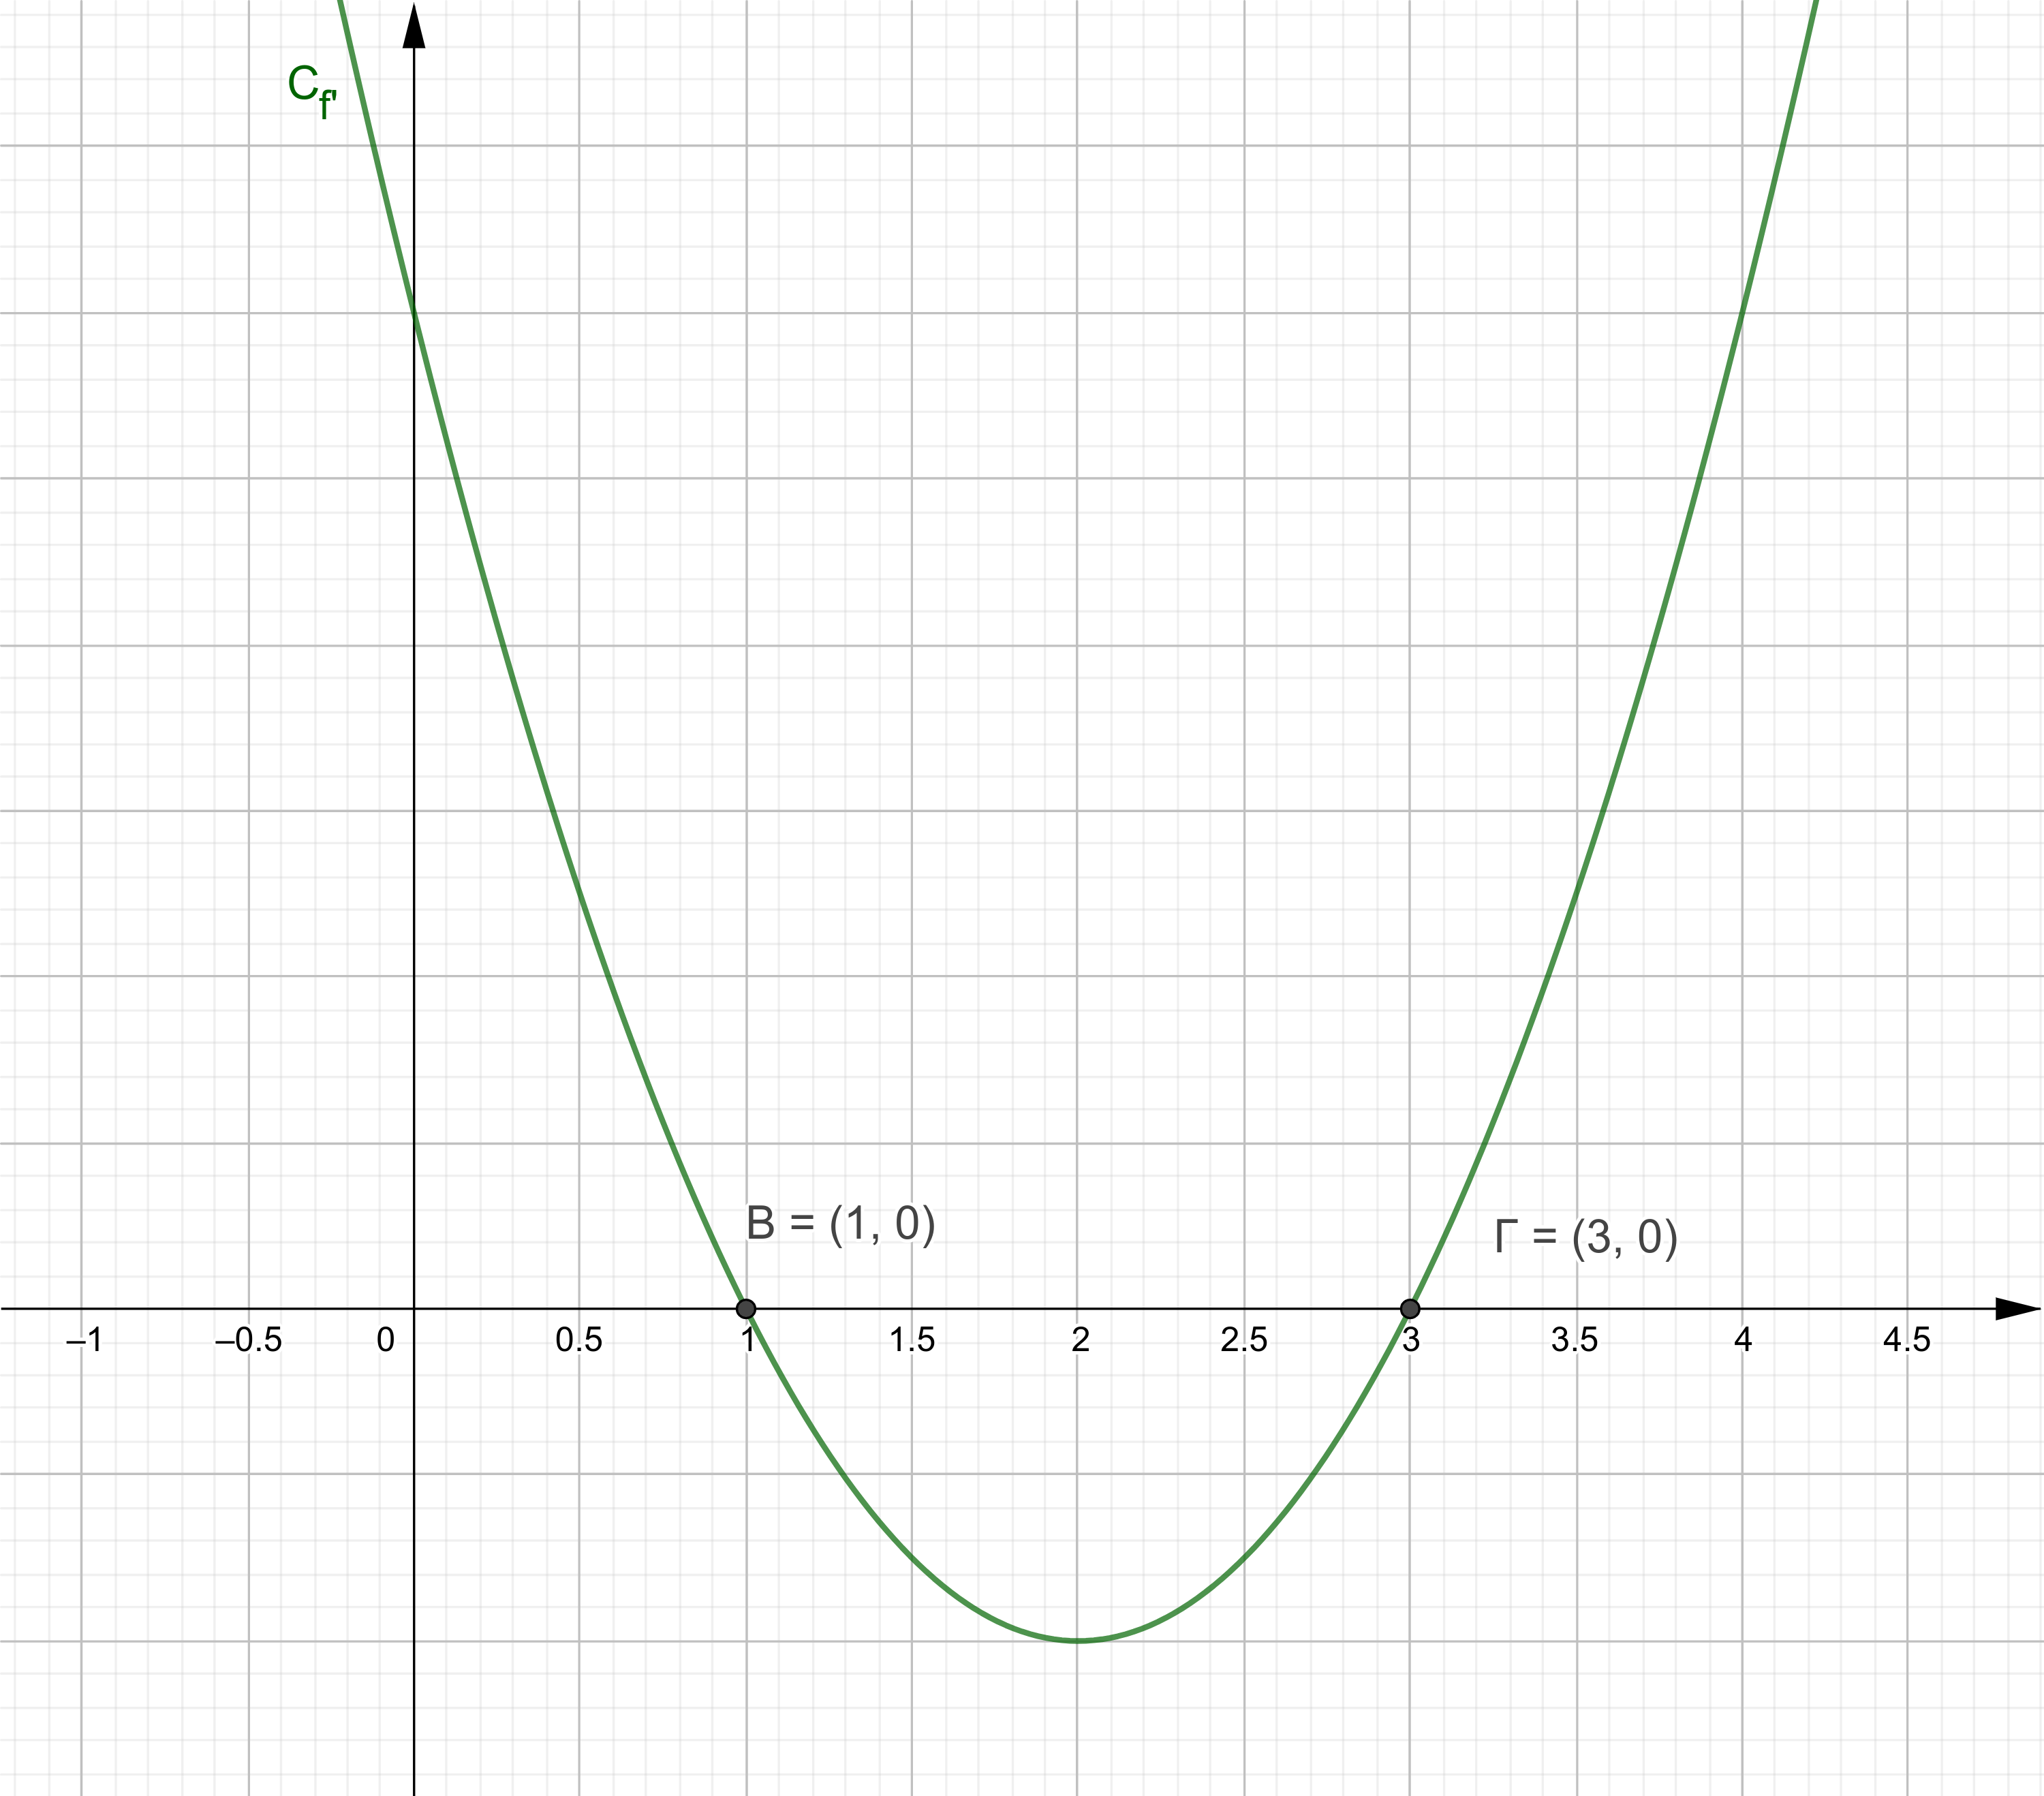
\includegraphics[width=0.3\textwidth]{2021Prosomeivsi2.png}
 \centering
\end{figure}
\begin{enumerate}
 \item[Β1.] \textbf{[Μονάδες 5]} Να βρείτε τα διαστήματα μονοτονίας και κυρτότητας για τη συνάρτηση $f$ καθώς επίσης τις θέσεις, το είδος των τοπικών ακροτάτων της και τη θέση που η $f$ έχει καμπή.
       
       Αν η $f$ είναι πολυωνυμική 3ου βαθμού και τέμνει τον άξονα $y'y$ σε σημείο με τεταγμένη $-2$, να δείξετε ότι:
       
 \item[Β2.] \textbf{[Μονάδες 7]} $f(x)=x^3-6x^2+9x-2$.
 \item[Β3.]
       \begin{enumerate}
        \item[i.] \textbf{[Μονάδες 3]} η $f$ παρουσιάζει δύο ακρότατα και ένα σημείο καμπής από τα οποία τα δύο από αυτά είναι συμμετρικά ως προς το τρίτο.
        \item[ii.] \textbf{[Μονάδες 5]} Η ευθεία $y=-3x+6$ "διαπερνά" την $C_f$
       \end{enumerate}
 \item[Β4.] \textbf{[Μονάδες 5]} $2f(2021)<f(2020)+f(2022)$.
\end{enumerate}

\section*{Θέμα Γ (24)}
Δίνεται η μοναδιαίος κύκλος κέντρου $Ο$ όπως φαίνεται στο σχήμα. Η ευθεία $(ε)$ είναι κάθετη στον άξονα $x'x$ στο σημείο $Α(1,0)$ και η γωνία $\widehat{ΑΟΜ}=θ$rad με $θ\in(-π,π)$ όπου $Μ$ σημείο του κύκλου. Έστω $Β(-1,0)$ και $ΒΜ$ τέμνει την $(ε)$ στο σημείο $Ν(1,y)$.
\begin{figure}[H]
 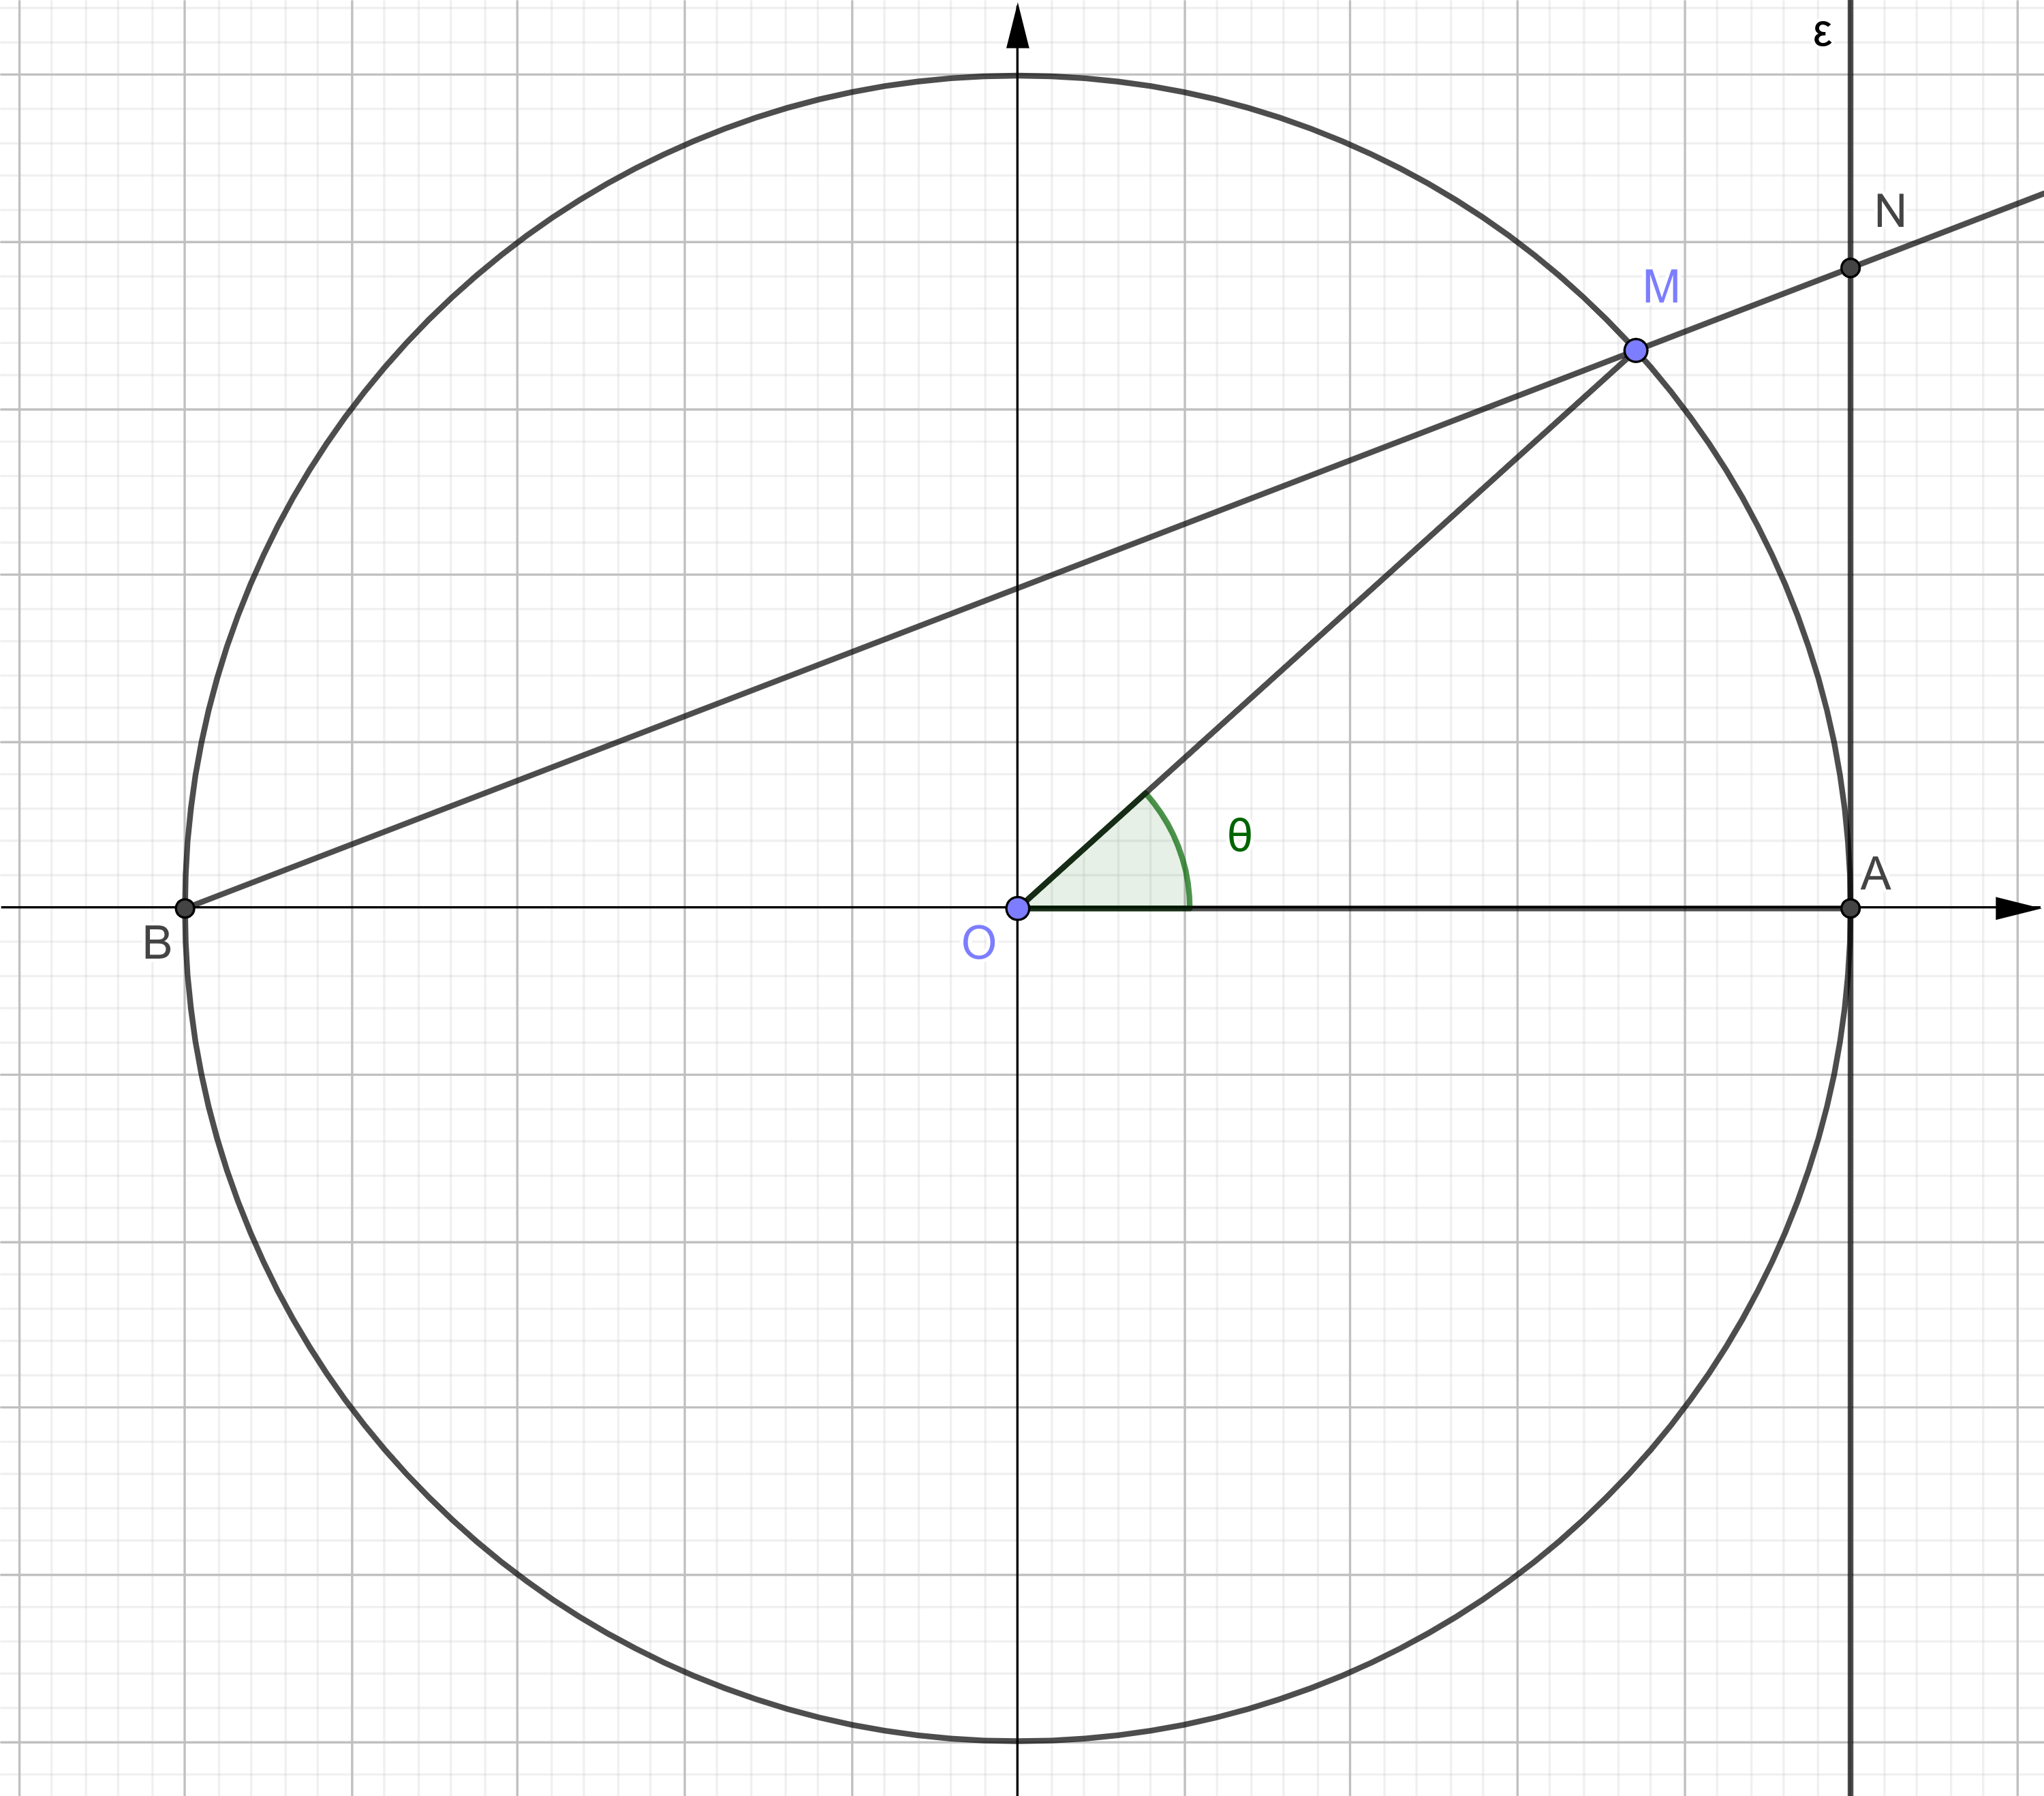
\includegraphics[width=0.35\textwidth]{2021Prosomeivsi.png}
 \centering
\end{figure}
\begin{enumerate}
 \item[Γ1.] \textbf{[Μονάδες 9]} Να δείξετε ότι $y=\frac{2ημθ}{1+συνθ}=y(θ)$.
 \item[Γ2.] \textbf{[Μονάδες 8]} Να βρείτε το
       \begin{enumerate}
        \item[i.] \textbf{[Μονάδες 2]} $\lim_{θ\to 0}\frac{y(θ)}{θ}$
        \item[ii.] \textbf{[Μονάδες 6]} Να βρείτε το $\lim_{θ\to π^-}y(θ)$ και $\lim_{θ\to π^+}y(θ)$ χρησιμοποιώντας αλλαγή μεταβλητής, θέτοντας $θ=π+u$ και $θ=u-π$ αντίστοιχα.
       \end{enumerate}
 \item[Γ3.] \textbf{[Μονάδες 6]} Να αποδείξετε ότι η συνάρτηση $y$ είναι περιττή και να τη μελετήσετε ως προς τη μονοτονία της.
 \item[Γ4.] \textbf{[Μονάδες 2]} Να βρείτε την εξίσωση της εφαπτομένης της $C_f$ στο σημείο της $(0,y(0))$ και το σύνολο τιμών της συνάρτησης.
\end{enumerate}

\section*{Θέμα Δ (24)}
Έστω η συνάρτηση $f:(0,+\infty)$ που είναι γνήσια μονότονη, δύο φορές παραγωγίσιμη για την οποία ισχύουν:
$$f(x)\ge 0 \text{ για κάθε } x\ge 1$$
και
$$\frac{f(x)+e^x}{x}\le e^x \text{ για κάθε } x>0$$
\begin{enumerate}
 \item[Δ1.] \textbf{[Μονάδες 6]} Να δείξετε ότι η $f$ έχει μοναδική ρίζα την $x=1$ και ότι είναι γνήσια αύξουσα στο πεδίο ορισμού της.
 \item[Δ2.] \textbf{[Μονάδες 6]} Να δείξετε ότι η εφαπτόμενη της $f$ στο σημείο της $Α(1,f(1))$ είναι η ευθεία με εξίσωση $y=ex-e$.
       
       Ισχύει επιπλέον ότι $x^2f''(x)+e^x=x^2f'(x)+xe^x$ για κάθε $x>0$.
       
 \item[Δ3.] \textbf{[Μονάδες 8]} Να δειχθεί ότι η $f(x)=e^x\ln x$, $x>0$ και να βρεθεί το σύνολο τιμών της συνάρτησης.
 \item[Δ4.] \textbf{[Μονάδες 5]} Αν η εφαπτόμενη της $f$ στο $Α(1,f(1))$ και η $C_f$ έχουν και άλλο κοινό σημείο με τετμημένη $x_0\in (0,1)$ α δείξετε ότι υπάρχει $ξ\in (x_0,1)$ ώστε να ισχύει $f(ξ)+\frac{e^ξ}{ξ}=e$.
\end{enumerate}

\end{document}
